\documentclass[10pt,twocolumn]{article} 
\usepackage{simpleConference}
\usepackage{times}
\usepackage{graphicx}
\usepackage{dcolumn,tabularx,booktabs,tabulary}
\usepackage{multirow}
\usepackage{amssymb}
\usepackage{url,hyperref}
\usepackage{authblk}
\usepackage{amsmath}
\begin{document}

\title{Using Deep Learning Neural Networks and Candlestick Chart Representation to Predict Stock Market}



\author[1]{Rosdyana Mangir Irawan Kusuma}
\author[2]{Wei-Chun Kao}
\author[3]{Trang-Thi Ho}
\author[1]{Yu-Yen Ou}
\affil[1]{Department of Computer Science and Engineering, Yuan Ze University, Taoyuan, Taiwan Roc}
\affil[2]{Omniscient Cloud Technology}
\affil[3]{Department of Computer Science and Engineering, National Taiwan University of Science and Technology, Taipei, Taiwan Roc}
\renewcommand\Authands{ and }

\maketitle
\thispagestyle{empty}

\begin{abstract}
Stock market prediction is still a challenging problem because there are many factors effect to the stock market price such as company news and performance, industry performance, investor sentiment, social media sentiment and economic factors. This work explores the predictability in the stock market using Deep Convolutional Network and candlestick charts. The outcome is utilized to design a decision support framework that can be used by traders to provide suggested indications of future stock price direction. We perform this work using various types of neural networks like convolutional neural network, residual network and visual geometry group network. From stock market historical data, we converted it to candlestick charts. After that, these candlestick charts will be feed as input for training a Convolution neural network model. This Convolution neural network model will help us to analyze the patterns inside the candlestick chart and predict the future movements of stock market. Using Taiwan 50 and Indonesian 10 stock market historical time series data we can achieve a promising results- 92.2 \% and 92.1 \% accuracy for Taiwan and Indonesia stock market respectively. Our performance results significantly outperform the existing methods.
\end{abstract}


\section{Introduction}
\subsection{Background}
The stock market is something that cannot be separated from modern human life. The Investment in stock market is a natural thing done by people around the world. They set aside their income to try their luck by investing in stock market to generate more profit. Traders are more likely to buy a stock whose value is expected to increase in the future. On the other hand, traders are likely to refrain from buying a stock whose value is expected to fall in the future. Therefore, an accurate prediction for the trends in the stock market prices in order to maximize capital gain and minimize loss is urgent demand. Besides, stock market prediction is still a challenging problem because there are many factors effect to the stock market price such as company news and performance, industry performance, investor sentiment, social media sentiment and economic factors. According to Fama’s efficient market hypothesis, argued that stocks always trade at their fair value, making it impossible for investors to either purchase undervalued stocks or sell stocks for inflated prices\cite{malkiel1970efficient}. As such, it should be impossible to outperform the overall market through expert stock selection or market timing, and that the only way an investor can possibly obtain higher returns is by chance or by purchasing riskier investments. With the current technological advances, machine learning is a breakthrough in aspects of human life today and deep neural network has shown potential in many research fields. In this research, we apply different types of machine learning algorithms to enhance our performance result for stock market prediction using convolutional neural network, residual network, virtual geometry group network, k-nearest neighborhood and random forest.
\par
Dataset format in machine learning can be different. Many kind of dataset format such as text sequence, image, audio, video, from 1D (one dimension) to 3D (three dimension) can be applicable for machine learning. Taken as an example, the image is used not only as input for image classification, but also as an input to predict a condition. We take the example of Google DeepMind in their research in Alpha Go\cite{he2016deep}. Recently, they are successfully get a lot of attention in the research field. By using the image as their input, where the image represents a Go game board, which later this image dataset is used to predict the next step of the opponent in the Go game.
\par
On the other occasion, from historical data of stock market converted into audio wavelength using deep convolutional wave net architecture can be applied to forecast the stock market movement\cite{borovykhdilated}.
\par 
Our proposed method in this work is using a candlestick chart from Taiwan and Indonesia stock market to predict the price movement. We utilized  three trading period times to analyze the correlation between those period times with the result. Our proposed candlestick chart will represent the sequence of time series with and without the daily volume stock data. Our experiments conduct two kind of image sizes (i.e. 50 and 20 dimension) for candlestick chart to analyze the correlation of hidden pattern in various image size. Thereafter our dataset will be feed as input for several learning algorithms of random forest and k-nearest neighborhood as traditional machine learning, CNN, residual network and VGG network as our modern machine learning. The goal is to analyze the correlation of some parameters such as period time, image size, feature set with the movement of stock market to check whether it will be going up or going down in the next day.
\subsubsection{Candlestick Chart}
Candlestick chart is a style of financial chart used to describe the price movements for a given period of time. Candlestick chart is also called a Japanese candlestick chart because it has been developed in the 18th century by Munehisa Hooma, a Japanese rice trader of financial instruments \cite{morris2006candlestick}. Each candlestick typically shows one day of trading data, thus a month chart may show the 20 trading days as 20 candlestick charts. Candlestick chart is like a combination of line-chart and a bar-chart, while each bar represents all four important pieces of information for that trading day. It consists of the open, the close, the high and low price.
\par
Candlesticks are usually composed of the real body, an upper and a lower shadow. If the opening price is higher than the closing price, then the real body will filled by red or black color. Otherwise, the real body will be drawn with green or white color. The upper and a lower shadow represent the high and low price ranges within a specified time period. However, not all candlesticks have a shadow. The Figure \ref{fig:candlestickformation} given clear explanation about real body and the shadows in candlestick.
\begin{figure}
  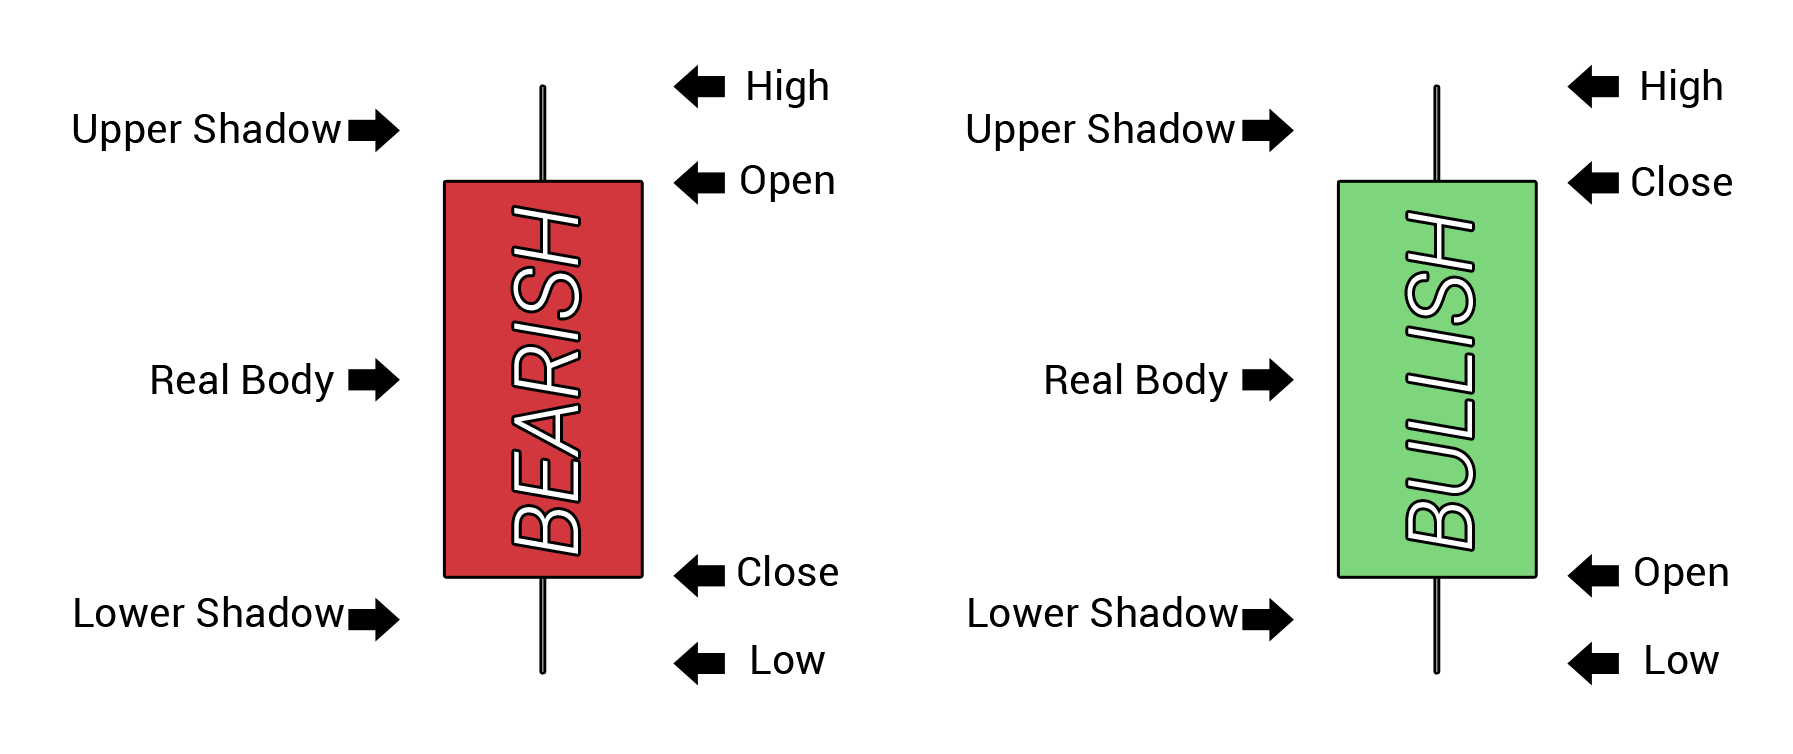
\includegraphics[width=\linewidth]{figures/candlestick_formation.png}
  \caption{Candlestick formation of bearish and bullish.}
  \label{fig:candlestickformation}
\end{figure}
\par
Candlestick chart are a visual aid for decision making in stock exchange. Each candlestick provides an easy-to-decipher picture of price action. Immediately a trader can compare the relationship between the open and close as well as the high and low. The relationship between the open and close is considered vital information and forms the essence of candlesticks. Bullish candlesticks, where the close is greater than the open, indicate buying pressure. Bearish candlesticks, where the close is less than the open, indicate selling pressure. It serves as a cornerstone of technical analysis. The main usage of a candlestick patterns is to identify trends. Looking at a candlestick, one can identify an asset’s opening and closing prices, highs and lows, and overall range for a specific time frame\cite{lu2012profitable}.

\subsection{Related Work}
There are many researchers have been started to develop the computational tool for the stock market prediction.$($ Schöneburg 1990 $)$ conducted a study using data from a randomly selected German stock market, then using the back-propagation method for their machine learning architecture \cite{schoneburg1990stock}. To our knowledge, stock market data consist of open price data, close price data, high price data, low price data and volume of the daily movement activity. In addition, to use the historical time series data from the stock market, some researchers in this field of stock market predictions began to penetrate the method of sentiment analysis to predict and analyze movements in the stock market.
\par
Bollen, Mao et al used their sentiment analysis method by taking data from one of the famous microblogging site Twitter to predict the Dow Jones Industrial Average $($DJIA$)$ stock market movements\cite{bollen2011twitter}. There are more studies on stock market predictions; they use the input data not only by using elements of historical time series data, but by also processing the data into other different forms. $($Borovykh, Bohte et al.$)$ tried to use the deep convolutional wave net architecture method to perform analysis and prediction using data from S \& P500 and CBOE \cite{borovykhdilated}.
\par
We also found some related work using candlestick charts in their research. $($do Prado, Ferneda et al. 2013$)$ used the candlestick chart to learn the pattern contained in Brazilian stock market by using sixteen candlestick patterns\cite{do2013effectiveness}. $($Tsai and Quan 2014$)$ utilized the candlestick chart to combine with seven different wavelet-based textures to analyze the candlestick chart\cite{tsai2014stock}. While,  $($Hu, Hu et al. 2017$)$ used the candlestick chart to build a decision-making system in stock market investment. They used the convolutional encoder to learn the patterns contained in the candlestick chart\cite{hu2017deep} while 
$($Patel, Shah et al. 2015$)$ used ten technical parameters from stock trading data for their input data and compare four prediction models, Artificial Neural Network $($ANN$)$, Support Vector Machine $($SVM$)$, random forest and naïve-Bayes\cite{patel2015predicting}. Traditional machine learning like Random Forest has been applied to predict the stock market with a good result. $($Khaidem, Saha et al. 2016$)$ combine the Random Forest with technical indicator such as Relative Strength Index $($RSI$)$ shown a good performance\cite{khaidem2016predicting}. Adding more feature set can be one of the way to enrich your dataset and enhance the result of classification. According to $($Zhang, Zhang et al. 2018$)$ input data not only from historical stock trading data, a financial news and users’ sentiments from social media can be correlated to predict the movement in stock market\cite{zhang2018improving}.
\par
Different from most of existing studies that only consider stock trading data, news events or sentiments in their models, our proposed method utilized a representation of candlestick chart images to analyze and predict the movement of stock market with a novel to compare modern and traditional neural network. 


\section{Data Collection}
\subsection{Data Collection using Yahoo! Finance}
Getting the right data in the right format is very important in machine learning because it will help our learning system go to right way and achieve a good result. Getting the right data means gathering or identifying the data that correlates with the outcomes you want to predict; i.e. data that contains a signal about events which you care about. The data needs to be aligned with the problem you are trying to solve. Example, the Kitten pictures are not very useful when you are building a facial identification system. A data scientist must do verifying that the data is aligned with the problem you are seeking to solve. If you do not have the right data, then your efforts to build an AI solution must return to the data collection stage.
Deep learning and machine learning more generally, needs a good training set to work properly. Collecting and constructing the training set – a sizable body of known data – takes time and domain-specific knowledge of where and how to gather relevant information. The training set acts as the benchmark against which deep-learning nets are trained. That is what they learn to reconstruct before they are unleashed on data which they have not seen before.
We trained and evaluated our model on two different stock markets, i.e. Taiwan and Indonesia. We collected 50 company stock markets for Taiwan and 10 company stock markets for Indonesia based on their growth in technical analysis as a top stock market in both countries.
\par
In this data collection, we use the application program interface $($API$)$ service from Yahoo! Finance to get historical time series data for each stock market shown in Figure \ref{fig:juvemarket}. From the period that we have been set in the following Table \ref{Tab:datasettime}, we certainly get some periods of trading day, starting from Monday until Friday is the period of trading day.

\begin{table}
    \caption{The period time of our dataset, separated between the training, testing and independent data.}
    \begin{tabularx}{\columnwidth}{X|X|X|X|X}
        \hline
        Stock Data	& Training Data    & Testing Data & Independent Data\\
        \hline
        TW50 & 2000/01/01 until 2016/12/31 & 2017/01/01 until 2018/06/14 & 2017/01/01 until 2018/06/14  \\
        ID10 & 2000/01/01 until 2016/12/31 & 2017/01/01 until 2018/06/14 & 2017/01/01 until 2018/06/14  \\
        \hline
    \end{tabularx}
    \label{Tab:datasettime}
\end{table}

\begin{figure}
  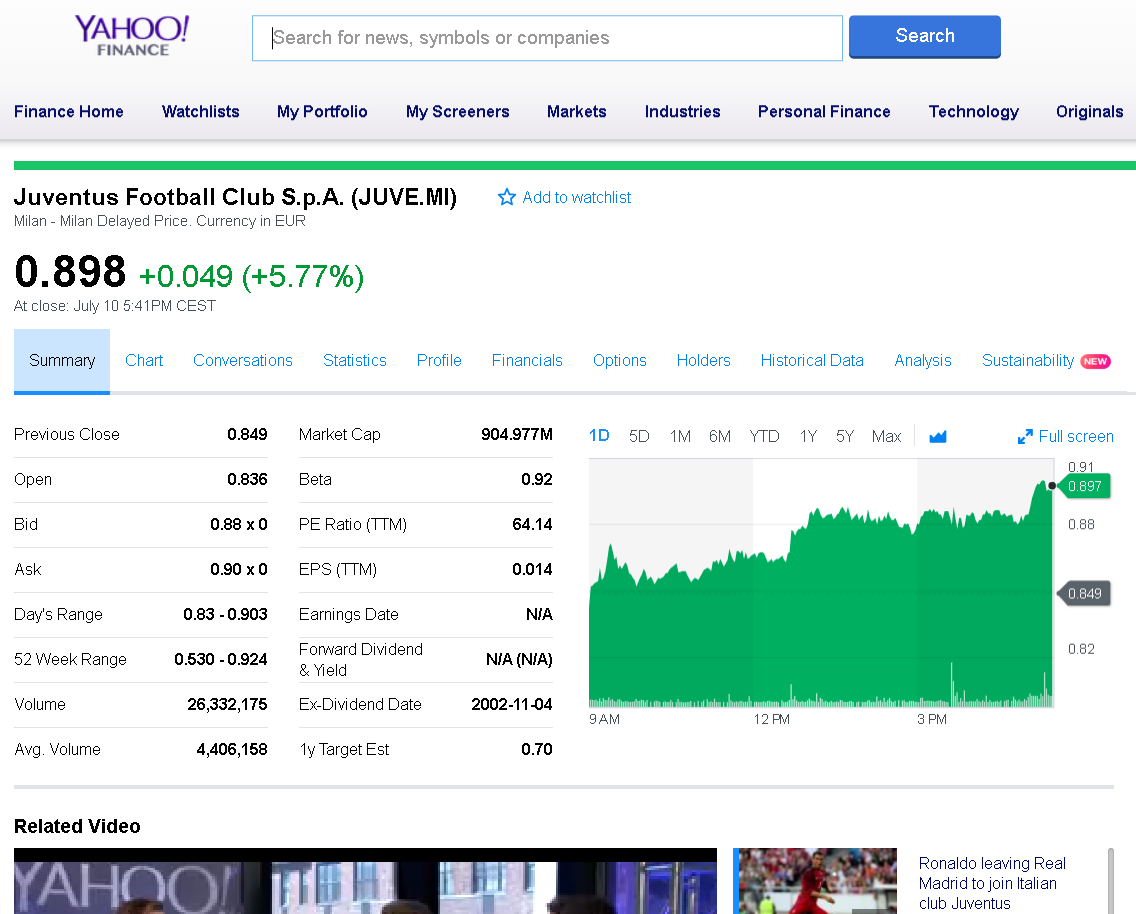
\includegraphics[width=\linewidth]{figures/juvemarket.png}
  \caption{Yahoo! Finance website, provide an API to download historical time series data.}
  \label{fig:juvemarket}
\end{figure}
\par
Segregation of data based on predetermined time for data training and data testing is important, while some studies make mistakes by scrambling data; this is certainly fatal because of the data, which we use, is time-series.

\subsection{Data Preprocessing}
We are processing our time series data using library Matplotlib \cite{hunter2007matplotlib} in python programming to convert from the historical data that we have prepared into a candlestick chart. We divide the period used to create candlestick chart based on 5 trading days’ data, 10 trading days’ data and 20 trading days’ data. 
The amount of data is shown in Table 6 can be different number because we will only generate a candlestick chart that is qualified based on the period set in the following Table \ref{Tab:datasettime}.

\begin{table}[htbp]
  \centering
  \caption{Add caption}
    \begin{tabular}{cD{,}{,}{3.7}D{,}{,}{5.1}}
    \toprule
    \textbf{Stock Data} & \multicolumn{2}{c}{\textbf{5 Period}} \\ \multicolumn{2}{c}{\textbf{10 Period}}\\
    \cmidrule{2-3}
     & \multicolumn{2}{c}{Carga Mineral (\%)} \\
     & \multicolumn{1}{c}{20}    &  \multicolumn{1}{c}{30} \\
     \midrule
    Fibra & 1,266 & 252 \\
    GCC & 0,316 & 52 \\
    Amido & 0,016 & 25 \\
    ASA & 0,002 & 252 \\
    Percol & 0,00032 & 25 \\
    \bottomrule
    \end{tabular}
  \label{tab_formacao_folhas2}%
\end{table}

\par
Besides the period time, we also divided our candlestick chart with and without volume indicator. The general candlestick chart usually only consists of time series data such as open price, close price, low price and high price shown in Figure \ref{fig:generalcandlestickchart}. Adding a volume indicator into candlestick chart is one of our approaches to find out correlation between enrich candlestick chart information and prediction result.
\begin{figure}
  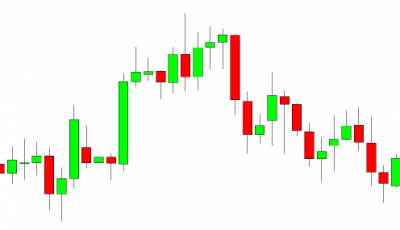
\includegraphics[width=\linewidth]{figures/generalcandlestickchart.png}
  \caption{General way to visualizing the candlestick chart.}
  \label{fig:generalcandlestickchart}
\end{figure}
\section{Methodology}
The architecture of our proposed stock market prediction is shown in Figure \ref{fig:methodologydesign}. The first, we collect the data from stock market historical data using Yahoo! Finance API. After that, we apply the sliding window technique to generate the period data before using computer graphic technique to generate the candlestick chart images. Finally, our candlestick charts are feed as input into some deep learning neural networks model for stock market prediction, and the outputs will be binary class to indicate the price will going up or down in the near future.
\begin{figure}
  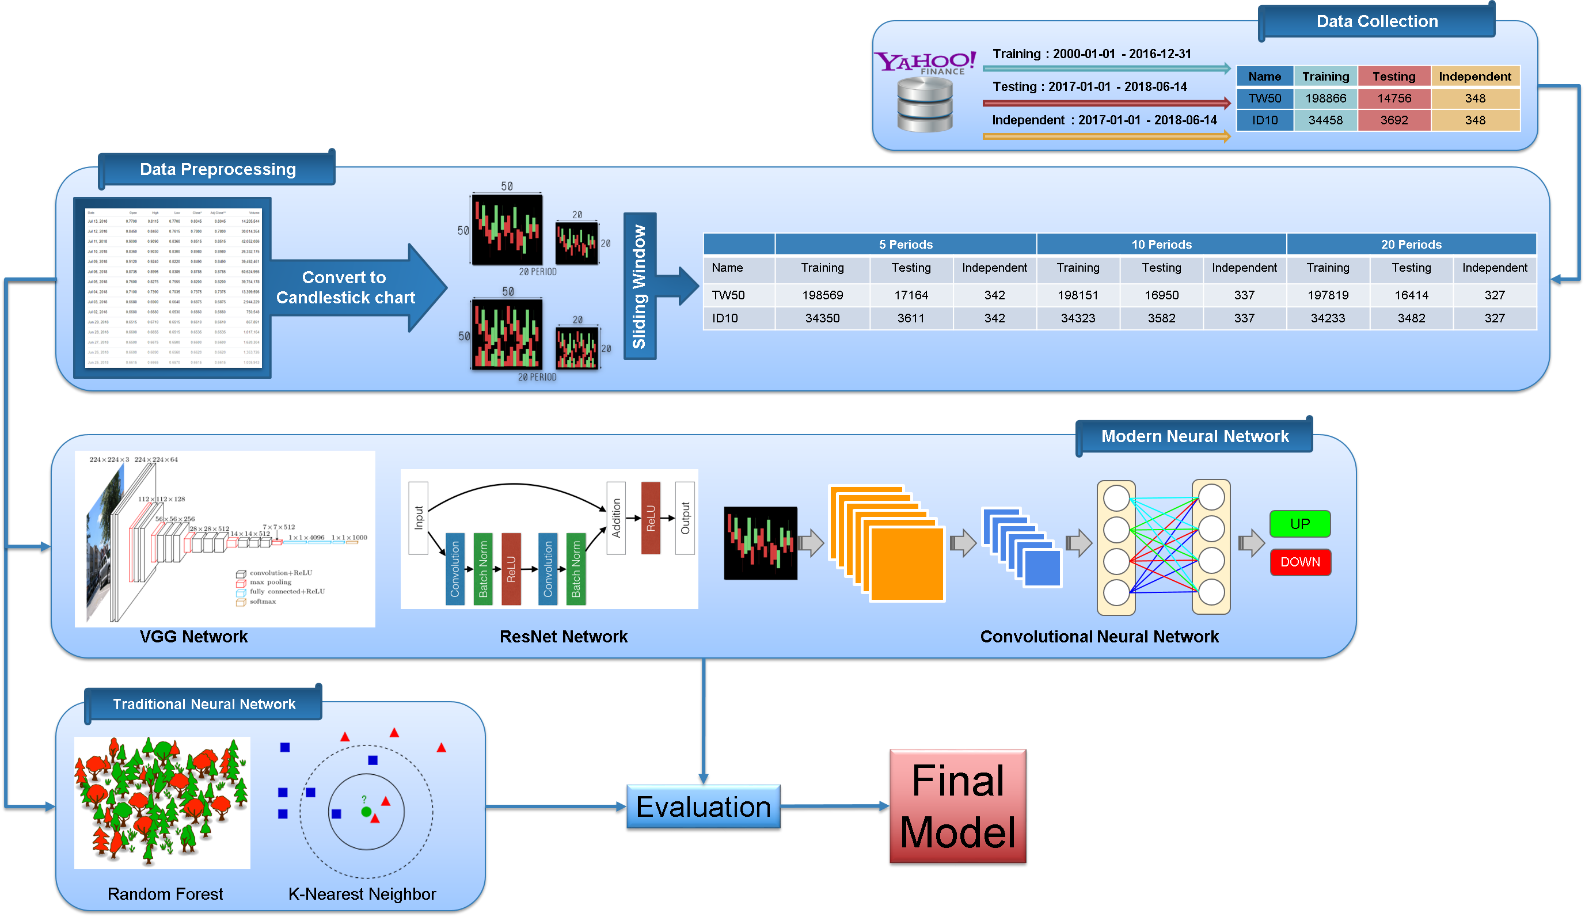
\includegraphics[width=\linewidth]{figures/methodology.png}
  \caption{Our methodology design.}
  \label{fig:methodologydesign}
\end{figure}
\subsection{Chart Encoding}
Candlesticks show that emotion by visually representing the size of price moves with different colors. Traders use the candlestick chart to make trading decision based on regularly occurring patterns that help forecast the short-term direction of the price. Just like a bar chart, a candlestick chart shows the stock market’s open price, high, low, and close price during those period time. The candlestick chart has a wide part, which is called body, the body represents the price range between the open and close of that day’s trading. When the body is filled in red, it means the close was lower than the open price. If the body is filled in green, it means the close was higher than the open price. 
We use computer graphics techniques implemented in python library called Matplotlib\cite{hunter2007matplotlib} to convert this time series data into a candlestick image size as 50x50 and 20x20 dimension with RGB$($Red Green Blue$)$ channel.
Figure \ref{fig:candlewithoutvolume} and Figure \ref{fig:candlewithvolume} describe our candlestick chart representation in different period time and size with volume and without volume respectively.
\begin{figure}
  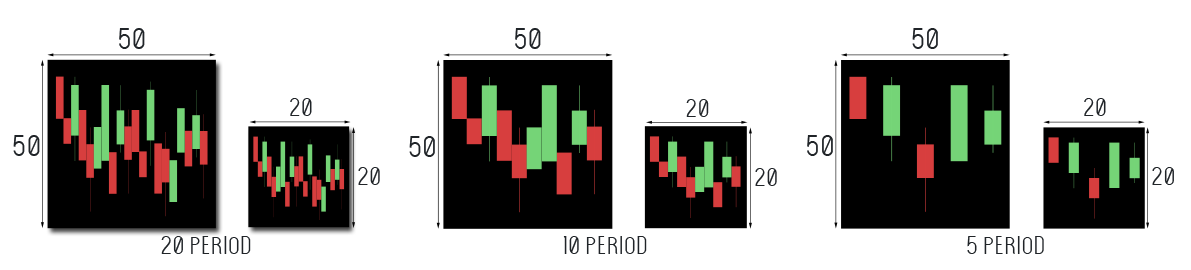
\includegraphics[width=\linewidth]{figures/candlewithoutvolume.png}
  \caption{Proposed candlestick chart without volume indicator in different period time and size.}
  \label{fig:candlewithoutvolume}
\end{figure}
\begin{figure}
  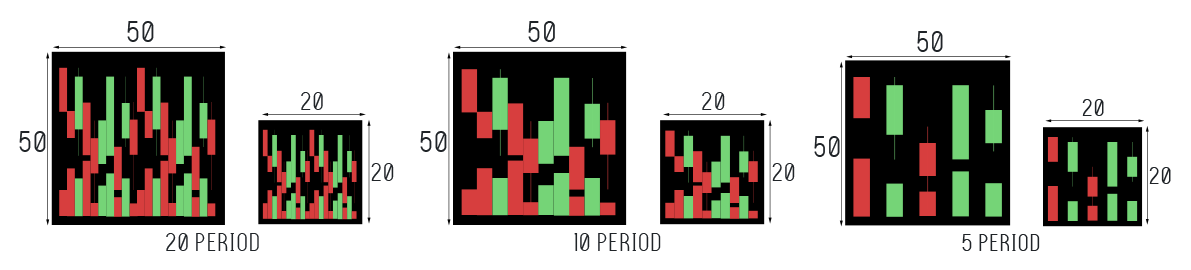
\includegraphics[width=\linewidth]{figures/candlewithvolume.png}
  \caption{Proposed candlestick chart with volume indicator in different period time and size.}
  \label{fig:candlewithvolume}
\end{figure}
\par
We utilized the black color as our candlestick chart background. For each candlestick chart, we configure the volume indicator shown a red bar if the closing price for the stock is lower than the opening price meaning negative volume, and green for days where the closing price is higher than opening price meaning positive volume.
\subsection{Learning Algorithm}
There is a lot of excitement surrounding the fields of Neural Networks (NN) and Deep learning (DL), due to numerous well-publicized successes that these systems have achieved in the last few years. We will use some Deep Learning Networks (DLN) based on Convolutional Neural Network to perform our classification on stock market prediction. Besides the DLN, we also apply some traditional Machine Learning (ML) algorithms to compare with DLN. Those traditional Machine Learning algorithms are Random Forest and K-Nearest Neighbors algorithms.
\subsubsection{Convolutional Neural Network}
Convolutional Neural Networks (CNNs) are very similar to ordinary Neural Networks (NN). They are made up of neurons with learnable weights and biases. Each neuron receives some inputs, performs a dot product and optionally follows it with a non-linearity. The whole network still expresses a single differentiable score function: from the raw image pixels on one end to class scores at the other. Moreover, they still have a loss function (e.g. SVM/Softmax) on the last (fully connected) layer and all the tips/tricks we developed for learning regular Neural Networks still apply.
As shown in Figure \ref{fig:simpleneuralnetwork}, Neural Networks receive an input (a single vector), and transform it through a series of hidden layers. Each hidden layer is made up of a set of neurons, where each neuron is fully connected to all neurons in the previous layer, and where neurons in a single layer function completely independently and do not share any connections. The last fully connected layer is called the “output layer” and in classification settings, it represents the class scores.
\begin{figure}
  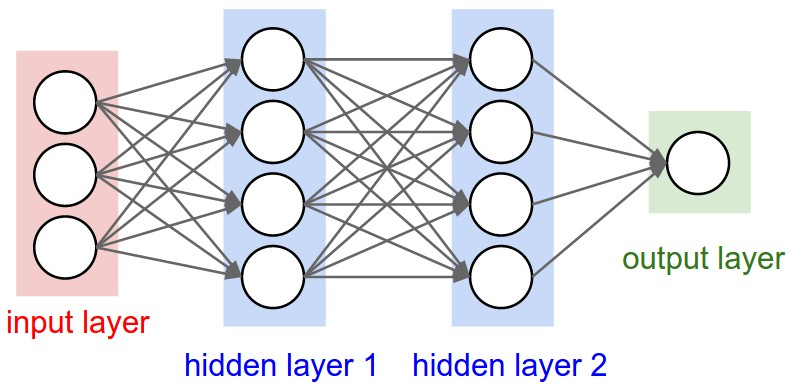
\includegraphics[width=\linewidth]{figures/simpleneuralnetwork.png}
  \caption{A regular 3-layer Neural Network.}
  \label{fig:simpleneuralnetwork}
\end{figure}
\par 
Our CNN model architecture consist of 4 layers of convolutional 2d, 4 layers of max pooling 2d, and 3 dropouts. The detail of CNN model architecture is shown in Table 7. The Conv layer is the core building block of a Convolutional Network that does most of the computational heavy lifting. The pool layers are in charge of down sampling the spatial dimensions of the input. The most common setting is to use max pooling with 2x2 receptive fields (i.e. F=2), and with a stride of two (i.e. S=2). Note that this discards exactly 75 \% of the activations in an input volume (due to down sampling by 2 in both width and height). Another slightly less common setting is to use 3x3 receptive fields with a stride of two, but this makes. It is very uncommon to see receptive field sizes for max pooling that are larger than three because the pooling is then too lossy and aggressive. This usually leads to worse performance.
\subsubsection{Residual Network}
Developed by He, Zhang et al. was the winner of ILSVRC 2015[15]. It features special skip connections and a heavy use of batch normalization. The architecture is also missing fully connected layers at the end of the network. ResNets are currently by far state of the art Convolutional Neural Network models
\par
As we have seen so far, increasing the depth should increase the accuracy of the network, as long as overfitting is taken care of. Nevertheless, the problem with increased depth is that the signal required to change the weights, which arises from the end of the network by comparing ground-truth and prediction becomes very small at the earlier layers, because of increased depth. It essentially means that earlier layers are almost negligible learned. This is called vanishing gradient.
\par 
The second problem with training the deeper networks is performing the optimization on huge parameter space and therefore naively adding the layers leading to higher training error. Residual networks allow training of such deep networks by constructing the network through modules called residual models.
\subsubsection{VGG Network}
The VGG network architecture was introduced by Simonyan and Zisserman[19]. It is named VGG because this architecture is from VGG group, Oxford. This network is characterized by its simplicity, using only 3x3 convolutional layers stacked on top of each other in increasing depth. Reducing volume size is handled by max pooling. Two fully connected layers, each with 4096 nodes are then followed by a softmax classifier shown in Table 9. The “16” and “19” stand for the number of weight layers in the network. Unfortunately, there are two major drawbacks with VGGNet. First, it is painfully slow to train and the second the network architecture weights themselves are quite large.
\subsubsection{Random Forest}
Random Forest classifier is a classifier with Consist of many decision trees and adopted the technique of random decision forest prioritizes predictive performance by using multiple learning algorithms (ensemble learning). In general, Decision trees are a learning methods used in data search technique. The method used by the idea of combining the "bagging" idea or called "Bootstrap Aggregating" (reduce variance) and the random selection of features in the training sets (classification and regression tree). 
Next we will bring more detail how we can use the various options in Random Forest usefully. Most of the options depend on two data objects generated by random forests. When the training set for the current tree is drawn by sampling with replacement, about one-third of the cases are left out of the sample. This OOB (out-of-bag) data is used to get a running unbiased estimate of the classification error as trees are added to the forest. It is also used to get estimates of variable importance. After each tree is built, all of the data are run down the tree, and proximities are computed for each pair of cases. If two cases occupy the same terminal node, their proximity is increased by one. At the end of the run, the proximities are normalized by dividing by the number of trees. Proximities are used in replacing missing data, locating outliers, and producing illuminating low-dimensional views of the data. 
The difference between Random Forest algorithm and the decision tree algorithm is that in Random Forest, the processes of finding the root node and splitting the feature nodes will run randomly. We applied our random forest algorithm from a machine learning python library called skicit-learn[20].
\subsubsection{K-Nearest Neighbors}
K-Nearest Neighbors (KNN) is a classifier with based on the Lazy learning and Instance-based (IBk) learning algorithms (selection K based value based on model evaluation method or cross validation). Further, Lazy learning is a learning method with the purposed to store training data and enables the training data is used when there is a query request is made (waits until it is given a test) by the system. Similarity measure applied to the KNN with the aim to compare every new case with available cases (training data) that has been previously saved. Conversely different with eager learning, eager learning is a learning method with the intention of preparing training process data earlier, then wait for the query request (a test). KNN implemented lazy learning method which has the distinct advantage that it can solve the problem by comparing the problem with similar past problem (case-based reasoning). KNN adopted a supervised learning approach by utilizing the data in this case must have class/label and this learning model of the algorithm can be used for classification and regression predictive problems.
We also using skicit-learn python library for our KNN classifier. Furthermore, we used a K-D Tree algorithm in our KNN to perform prediction with default parameter from scikit-learn library.
\subsection{Performance Evaluation}
There are some statistics measures of the performance evaluation to evaluate the result of all the classifiers by measuring the sensitivity (true positive rate or recall), specificity (true negative rate), accuracy and Matthew's correlation coefficient (MCC). In general, TP is true positive or correctly identified, FP is false positive or incorrectly identified, TN is true negative or correctly rejected and FN is false negative or incorrectly rejected. Formulated as follows:

\section{Experimental Results and Discussion}
\subsection{Classifiaction for Each Stock Market}
In this study, we try to make stock market predictions by using binary classification. Where the value 1 on the label means price increasing on the next day, while the value 0 is the reverse of it.
We trained and evaluated our binary classification model on two challenging datasets, i.e. Taiwan 50 and Indonesia 10 stock market. Taiwan 50 dataset includes 50 company stock markets from Taiwan and Indonesia 10 dataset includes 10 company stock markets from Indonesia which most of them are the top stock market in both countries. We also divide the retrieval period based on the duration of the 5 days, 10 days and 20 days of trading days to create a sequence of sliding windows that will be converted to candlestick chart. Another hands, we also generate the candlestick chart with and without volume indicator for 2 different image sizes, 50 and 20 dimension. 
\subsubsection{Classification for Taiwan 50 Dataset}
From all experiments about Taiwan 50, we conclude a summary result with and without volume indicator for different trading days’ period and image dimension result. Table 22 shows that CNN in 20 trading days’ period with 50-dimension image and volume indicator is better than the others with 91.5\% accuracy. In addition, without volume indicator for Taiwan 50, CNN in 20 trading days’ period with 50 dimension performs better than the others with 92.2\% accuracy. From the result of both of those experiments, it indicates that the method using CNN model with longer trading day’s period without volume indicator can achieve the best result for Taiwan 50 dataset.
\subsubsection{Classification for Indonesia 10 Dataset}
From all experiment results with Indonesia 10 dataset, we conclude a summary result with and without volume indicator in Tables 36 and 37 respectively. It shows that the CNN method with 20 trading days’ period in 50 dimension using volume indicator show the best result with 90.0\% accuracy in Table 37. While the CNN method in 20 trading days’ period with 20-dimension image without using the volume indicator performs better result with 92.1\% accuracy. It indicates that the method using CNN model with longer trading day’s period without volume indicator can achieve the best result for Indonesia 10 dataset.
\subsection{Independent Testing Result}
Measuring our model result not only used performance evaluation. We also performed an independent test to see that our proposed method is reasonable. During this independent test, we used two index stock exchange data from each country. Yuanta/P-shares Taiwan Top 50 ETF represented independent data test for our Taiwan50, whereas Jakarta Composite Index is our independent data set test for Indonesia10. Both of the stock exchange data are taken from 1st January, 2017 until 14th June 2018. 
Tables 38 and 39 show our independent test result for Taiwan50 using volume indicator and without using volume indicator respectively. The independent test result for Indonesia10 using and without using volume indicator are shown in Tables 40 and 41 respectively. As shown in Tables 38, 39, 40 and 41, our CNN with 20 trading days’ period and 50-dimension image get best result for both independent test. It indicated again that our proposed method outperforms the others.
\subsection{Comparison}
To further evaluate the effectiveness of our predictive model, we also compare our result with the other related works. The first comparison is between our proposed method with [12], they used three different stock market datasets with different trading period time. Samsung, General Electric and Apple are their stock market data with one, two and three months of trading period respectively. We applied our proposed model in their datasets to compare our prediction performance with their result shown in [12]. The comparison result for Samsung, Apple, and GE stock market shown in Table 42, 43, and 44 respectively. Based on these comparison results, it revealed that our performance results outperformed the prediction results from [12].

\section{Conclusions and Future Works}

In this study, we present a new method for stock market prediction using 2 stock market datasets including 50 company stock markets for Taiwan50 datasets and 10 company stock market for Indonesian datasets. The first, we employ the sliding window technique to generate the period data. To find out correlation between enrich candlestick chart information and stock market prediction performance, we utilized the computer graphic technique to generate the candlestick chart images for stock market data. Finally, an CNN learning algorithm is employed to build our prediction for stock market.
\par
We found that the model using long-term trading days’ period with CNN learning algorithm achieves the highest performance of sensitivity, specificity, accuracy, and MCC. It is proved that Convolutional neural network can find the hidden pattern inside the candlestick chart images to forecast the movement of specific stock market in the future. Adding the indicator such as volume in candlestick chart not really help the algorithms increase finding the hidden pattern.
\par
The comparison experiments indicated that our proposed method provide highly accurate forecast for other datasets compare to the other existing methods. Patel used trading data from Reliance Industries, Infosys Ltd., CNX Nifty and S\&\P Bombay Stock Exchange BSE Sensex during 10 years with accuracy in the range of 89 – 92 \% while we achieved accuracy in the range of 93 – 97 \%. Khaidem method achieved the accuracy in the range of 86 – 94 \% using three trading data from Samsung, GE and Apple while we achieved in the range of 87 – 97 \%. Zhang utilized 13 different companies in Hong Kong stock exchange with accuracy 61 \%. Meanwhile, our method achieved 92 \% for accuracy. 
\par
For the future works we want to extend our work being able to predict the percentage change on the price movements. For the convenience of experimental scientists, we developed a user-friendly webserver for predicting stock market using our final model. Available at http://140.138.155.216/deepcandle, DeepCandle is a system through which users can easily predicting stock market in the near future. Users only need to input the date target, and our models will process them and return a summary. The provided web interface is constructed such that users can easily access its functions and comfortably use it without a deep understanding of computing.


\bibliographystyle{abbrv}
\bibliography{refs}
\end{document}
